\begin{frame}
	\myheading{Module 10.5: Skip-gram model}
\end{frame}

\begin{frame}
	\begin{block}{}
		\onslide<1-2>
		\begin{itemize}
			\justifying
			\item<1-> The model that we just saw is called the continuous bag of words model (it predicts an output word give a bag of context words)
			\item<2-> We will now see the skip gram model (which predicts context words given an input word)
		\end{itemize}
	\end{block}
\end{frame}


\begin{frame}
	\begin{columns}
		\column{0.5\textwidth}
		\begin{overlayarea}{\textwidth}{\textheight}
			\begin{tikzpicture}

\node (R)[text width=\textwidth] at (0,3) {\footnotesize{\begin{table}
\begin{tabular}{|c|c|c|c|c|c|c|}
\hline
0 & 0 & 1 & ... & 0 & 0 & 0\\
\hline
\end{tabular}
\end{table}}
};
\node (H) [text width=\textwidth] at ($ (R) + (0,2) $) {\begin{table}
\begin{tabular}{l!{\color{white}\vrule}l!{\color{white}\vrule}l!{\color{white}\vrule}l!{\color{white}\vrule}l!{\color{white}\vrule}l!{\color{white}\vrule}l!{\color{white}\vrule}l!{\color{white}\vrule}l!{\color{white}\vrule}l}
\hline
\rowcolor{blue!50}
 .&.&.&.&.&.&.&.&.&.\\
\hline
\end{tabular}
\end{table}
};

\draw [fill=red!50] ($(H) + (-3.75,1.5)$) rectangle ($ (H) + (-2.25, 1.8)$);
\draw [fill=red!50] ($(H) + (-1.75,1.5)$) rectangle ($ (H) + (-0.25, 1.8)$);
\draw [fill=red!50] ($(H) + (0.25,1.5)$) rectangle ($ (H) + (1.75, 1.8)$);
\draw [fill=red!50] ($(H) + (2.25,1.5)$) rectangle ($ (H) + (3.75, 1.8)$);
\onslide<1,3->{
\node [color=red!50] at ($ (H) + (-3,2)$) {\textit{he}};
\node[color=red!50] at ($ (H) + (-1,2)$) {\textit{sat}};
\node[color=red!50] at ($(H) + (1,2)$) {\textit{a}};
\node[color=red!50] at ($(H) + (3,2)$) {\textit{chair}};
}
\onslide<2>{
\node [color=black!10] at ($ (H) + (-3,2)$) {\textit{he}};
\node[color=red!50] at ($ (H) + (-1,2)$) {\textit{sat}};
\node[color=black!10] at ($(H) + (1,2)$) {\textit{a}};
\node[color=black!10] at ($(H) + (3,2)$) {\textit{chair}};
}
\if 0
\node(V) [text width=\textwidth] at ($ (H) + (0,1.5) $) {\large{\begin{table}
\begin{tabular}{l!{\color{white}\vrule}l!{\color{white}\vrule}l!{\color{white}\vrule}l!{\color{white}\vrule}l!{\color{white}\vrule}l!{\color{white}\vrule}l!{\color{white}\vrule}l!{\color{white}\vrule}l!{\color{white}\vrule}l!{\color{white}\vrule}l!{\color{white}\vrule}l}
\hline
\rowcolor{red!50}
 .&.&.&.&.&.&.&.&.&.&.&.\\
\hline
\end{tabular}
\end{table}}
};
 
\node[text width=0.15\textwidth, rotate=90] at ($(V) + (-3,0.9)$ ) {\tiny{$P(he|sat)$}};
\node[text width=0.15\textwidth, rotate=90] at ($(V) + (-2.5,0.9)$ ) {\tiny{$P(chair|sat)$}};
\node[text width=0.15\textwidth, rotate=90] at ($(V) + (-2.0,0.9)$ ) {\tiny{$P(man|sat)$}};
\node[text width=0.15\textwidth, rotate=90] at ($(V) + (1.4,0.9)$ ) {\tiny\textcolor{red}{{$P(on|sat)$}}};
\fi

%\draw[line width=1][->] (0,1.6) -- (0,2.75);
\node[text width=0.3\textwidth, ] at ($(H) + (3.8,0)$ ) {\tiny{$\mathbf{h} \in \mathbb{R}^{|k|}$}};
\node[text width=0.3\textwidth, ] at ($(H) + (2.5,0.7)$ ) {\tiny{$W_{context} \in \mathbb{R}^{k\times |V|}$}};
\node[text width=0.3\textwidth, ] at ($(0,2.7) + (3.3,0.4)$ ) {\tiny{$\mathbf{x} \in \mathbb{R}^{|V|}$}};
\node[text width = 0.3\textwidth] at (0.7, 4){\tiny{$W_{word} \in \mathbb{R}^{k\times |V|}$}};
\draw[line width=0.5] (-2.15,3.15) -- (-2.7,4.7);
\draw[line width=0.5] (2.15,3.15) -- (2.7,4.7);

\draw[line width=0.5] [->](0,5.20) -- ($(H) + (-3,1.5)$);
\draw[line width=0.5] [->] (0,5.20) -- ($(H) + (3,1.5)$);
\draw[line width=0.5] [->] (0,5.20) -- ($(H) + (-1,1.5)$);
\draw[line width=0.5] [->] (0,5.20) -- ($(H) + (1,1.5)$);
\end{tikzpicture}

		\end{overlayarea}
		\column{0.5\textwidth}
		\begin{overlayarea}{\textwidth}{\textheight}
			\onslide<1-4>{
				\begin{itemize}
					\justifying
					\item<1-> Notice that the role of $context$ and $word$ has changed now
					\item<2-> In the simple case when there is only one $context$ word, we will arrive at the same update rule for $u_c$ as we did for $v_w$ earlier
					\item<3-> Notice that even when we have multiple context words the loss function would just be a summation of many cross entropy errors
					      \begin{align*}
						      \mathscr{L}(\theta) & = - \sum_{i=1}^{d-1} \log \hat{y}_{w_i}
					      \end{align*}
					\item<4-> Typically, we predict context words on both sides of the given word
				\end{itemize}}
		\end{overlayarea}
	\end{columns}
\end{frame}

\begin{frame}
	\begin{columns}
		\column{0.5\textwidth}
		\begin{overlayarea}{\textwidth}{\textheight}
			\begin{tikzpicture}

\node (R)[text width=\textwidth] at (0,3) {\footnotesize{\begin{table}
\begin{tabular}{|c|c|c|c|c|c|c|}
\hline
0 & 0 & 1 & ... & 0 & 0 & 0\\
\hline
\end{tabular}
\end{table}}
};
\node (H) [text width=\textwidth] at ($ (R) + (0,2) $) {\begin{table}
\begin{tabular}{l!{\color{white}\vrule}l!{\color{white}\vrule}l!{\color{white}\vrule}l!{\color{white}\vrule}l!{\color{white}\vrule}l!{\color{white}\vrule}l!{\color{white}\vrule}l!{\color{white}\vrule}l!{\color{white}\vrule}l}
\hline
\rowcolor{blue!50}
 .&.&.&.&.&.&.&.&.&.\\
\hline
\end{tabular}
\end{table}
};

\draw [fill=red!50] ($(H) + (-3.75,1.5)$) rectangle ($ (H) + (-2.25, 1.8)$);
\draw [fill=red!50] ($(H) + (-1.75,1.5)$) rectangle ($ (H) + (-0.25, 1.8)$);
\draw [fill=red!50] ($(H) + (0.25,1.5)$) rectangle ($ (H) + (1.75, 1.8)$);
\draw [fill=red!50] ($(H) + (2.25,1.5)$) rectangle ($ (H) + (3.75, 1.8)$);
\node [color=red!50] at ($ (H) + (-3,2)$) {\textit{he}};
\node[color=red!50] at ($ (H) + (-1,2)$) {\textit{sat}};
\node[color=red!50] at ($(H) + (1,2)$) {\textit{a}};
\node[color=red!50] at ($(H) + (3,2)$) {\textit{chair}};
\if 0
\node(V) [text width=\textwidth] at ($ (H) + (0,1.5) $) {\large{\begin{table}
\begin{tabular}{l!{\color{white}\vrule}l!{\color{white}\vrule}l!{\color{white}\vrule}l!{\color{white}\vrule}l!{\color{white}\vrule}l!{\color{white}\vrule}l!{\color{white}\vrule}l!{\color{white}\vrule}l!{\color{white}\vrule}l!{\color{white}\vrule}l!{\color{white}\vrule}l}
\hline
\rowcolor{red!50}
 .&.&.&.&.&.&.&.&.&.&.&.\\
\hline
\end{tabular}
\end{table}}
};
 
\node[text width=0.15\textwidth, rotate=90] at ($(V) + (-3,0.9)$ ) {\tiny{$P(he|sat)$}};
\node[text width=0.15\textwidth, rotate=90] at ($(V) + (-2.5,0.9)$ ) {\tiny{$P(chair|sat)$}};
\node[text width=0.15\textwidth, rotate=90] at ($(V) + (-2.0,0.9)$ ) {\tiny{$P(man|sat)$}};
\node[text width=0.15\textwidth, rotate=90] at ($(V) + (1.4,0.9)$ ) {\tiny\textcolor{red}{{$P(on|sat)$}}};
\fi

%\draw[line width=1][->] (0,1.6) -- (0,2.75);
\node[text width=0.3\textwidth, ] at ($(H) + (3.8,0)$ ) {\tiny{$\mathbf{h} \in \mathbb{R}^{|k|}$}};
\node[text width=0.3\textwidth, ] at ($(H) + (2.5,0.7)$ ) {\tiny{$W_{context} \in \mathbb{R}^{k\times |V|}$}};
\node[text width=0.3\textwidth, ] at ($(0,2.7) + (3.3,0.4)$ ) {\tiny{$\mathbf{x} \in \mathbb{R}^{|V|}$}};
\node[text width = 0.3\textwidth] at (0.7, 4){\tiny{$W_{word} \in \mathbb{R}^{k\times |V|}$}};
\draw[line width=0.5] (-2.15,3.15) -- (-2.7,4.7);
\draw[line width=0.5] (2.15,3.15) -- (2.7,4.7);

\draw[line width=0.5] [->](0,5.20) -- ($(H) + (-3,1.5)$);
\draw[line width=0.5] [->] (0,5.20) -- ($(H) + (3,1.5)$);
\draw[line width=0.5] [->] (0,5.20) -- ($(H) + (-1,1.5)$);
\draw[line width=0.5] [->] (0,5.20) -- ($(H) + (1,1.5)$);
\end{tikzpicture}

		\end{overlayarea}
		\column{0.5\textwidth}
		\begin{overlayarea}{\textwidth}{\textheight}
			\onslide<1->{
				\textbf{Some problems}
				\begin{itemize}\justifying
					\item<1-> Same as bag of words
					\item<2-> The softmax function at the output is computationally expensive
					\item<3-> \textcolor<6->{red}{Solution 1: Use negative sampling}
					\item<4-> Solution 2: Use contrastive estimation
					\item<5-> Solution 3: Use hierarchical softmax
				\end{itemize}
			}
		\end{overlayarea}
	\end{columns}
\end{frame}


\begin{frame}
	\begin{columns}
		\column{0.35\textwidth}
		\begin{overlayarea}{\textwidth}{\textheight}

			\begin{itemize}
				\justifying
				\onslide<1->{\item $D$ = [(sat, on), (sat, a), (sat, chair), (on, a), (on,chair), (a,chair),
				      (on,sat), (a, sat), (chair,sat), (a, on), (chair, on), (chair, a) ]
				      }
				      \vspace{0.1in}
				      \onslide<2->{\item $D^{'}$ = [(sat, oxygen), (sat, magic), (chair, sad), (chair, walking)]
				      }
			\end{itemize}
		\end{overlayarea}
		\column{0.65\textwidth}
		\begin{overlayarea}{\textwidth}{\textheight}
			\onslide<1-4>{
				\begin{itemize}\justifying
					\item<1-> Let $D$ be the set of all correct $(w,c)$ pairs in the corpus
					\item<2-> Let $D^{'}$ be the set of all incorrect $(w,r)$ pairs in the corpus
					\item<3-> $D^{'}$ can be constructed by randomly sampling a context word $r$ which has
					      never appeared with $w$ and creating a pair $(w, r)$
					\item<4-> As before let $v_w$ be the representation of the word $w$ and $u_c$ be the
					      representation of the context word $c$
				\end{itemize}}
		\end{overlayarea}
	\end{columns}
\end{frame}

\begin{frame}
	\begin{columns}
		\column{0.35\textwidth}
		\begin{overlayarea}{\textwidth}{\textheight}
			\vspace{0.2in}
			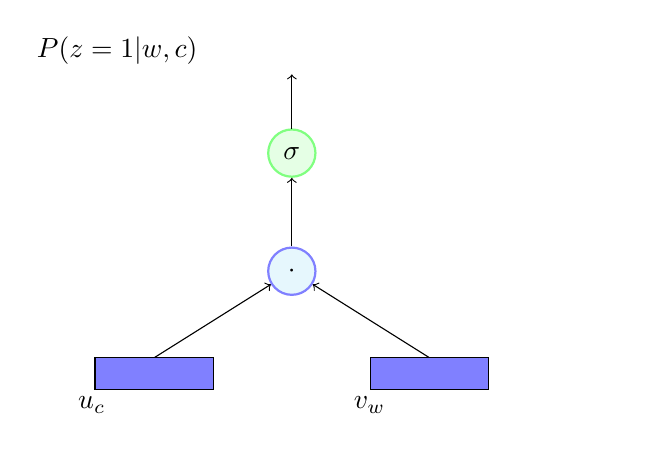
\begin{tikzpicture}
				\tikzstyle{hidden_neuron}=[circle,draw=blue!50,fill=cyan!10,thick,minimum size=6mm]
				\tikzstyle{output_neuron}=[circle,draw=green!50,fill=green!10,thick,minimum size=6mm]
				\node [hidden_neuron] (n1) at (0,1.5){$\cdot$};
				\node [output_neuron] (n2) at (0,3){$\sigma$};
				\draw [->] (0,3.3) -- (0,4);
				\draw [->] (-1.75,0.4) -- (n1);
				\draw [->] (1.75,0.4) -- (n1);
				\node [text width=0.6\textwidth] at (0.4,4.3) {$P(z=1|w,c)$};
				\draw [->] (n1) -- (n2);
				\draw [fill=blue!50] (-2.5, 0) rectangle (-1,0.4);
				\draw [fill=blue!50] (1, 0) rectangle (2.5,0.4);
				\node [text width=0.2\textwidth] at (-1.5,-0.2){$u_c$};
				\node [text width=0.2\textwidth] at (2,-0.2){$v_w$};
			\end{tikzpicture}
		\end{overlayarea}
		\column{0.65\textwidth}
		\begin{overlayarea}{\textwidth}{\textheight}
			\onslide<1-3>{
				\begin{itemize}
					\justifying
					\item<1-> For a given $(w,c) \in D$ we are interested in maximizing
					      \begin{align*}
						      p(z = 1| w,c)
					      \end{align*}
					\item<2-> Let us model this probability by
					      \begin{align*}
						      p(z=1|w,c) & = \sigma(u_c^T v_w)\\
						      & = \frac{1}{1 + e^{-u_c^{T}v_w}}
					      \end{align*}
					\item<3-> Considering all $(w,c) \in D$, we are interested in
					      \begin{align*}
						      \underset{\theta}{maximize} \underset{(w,c) \in D}{\prod}p(z=1|w,c)
					      \end{align*}
					      where $\theta$ is the word representation ($v_w$)
					      and context representation ($u_c$) for all words in our corpus
				\end{itemize}}
		\end{overlayarea}
	\end{columns}
\end{frame}


\begin{frame}
	\begin{columns}
		\column{0.35\textwidth}
		\begin{overlayarea}{\textwidth}{\textheight}
			\vspace{0.2in}
			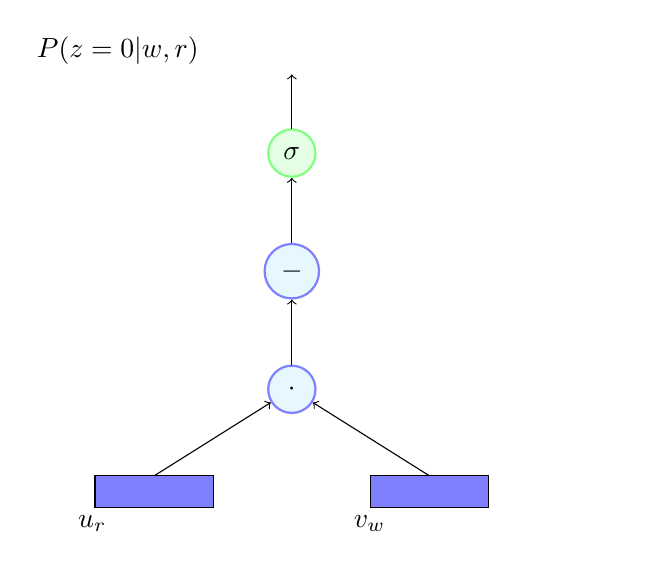
\begin{tikzpicture}
				\tikzstyle{hidden_neuron}=[circle,draw=blue!50,fill=cyan!10,thick,minimum size=6mm]
				\tikzstyle{output_neuron}=[circle,draw=green!50,fill=green!10,thick,minimum size=6mm]
				\node [hidden_neuron] (n1) at (0,1.5){$\cdot$};
				\node [hidden_neuron] (n2) at (0,3){$-$};
				\node [output_neuron] (n3) at (0,4.5){$\sigma$};
				\draw [->] (0,4.8) -- (0,5.5);
				\draw [->] (-1.75,0.4) -- (n1);
				\draw [->] (1.75,0.4) -- (n1);
				\node [text width=0.6\textwidth] at (0.4,5.8) {$P(z=0|w,r)$};
				\draw [->] (n1) -- (n2);
				\draw [->] (n2) -- (n3);
				\draw [fill=blue!50] (-2.5, 0) rectangle (-1,0.4);
				\draw [fill=blue!50] (1, 0) rectangle (2.5,0.4);
				\node [text width=0.2\textwidth] at (-1.5,-0.2){$u_{r}$};
				\node [text width=0.2\textwidth] at (2,-0.2){$v_w$};
			\end{tikzpicture}
		\end{overlayarea}
		\column{0.65\textwidth}
		\begin{overlayarea}{\textwidth}{\textheight}
			\begin{itemize}
				\justifying
				\onslide<1->{\item For $(w,r) \in D^{'}$ we are interested in maximizing}
				      \begin{align*}
					      \onslide<1->{  p(z = 0| w,r)}
				      \end{align*}
				      \onslide<2->{\item Again we model this as}
				      \begin{align*}
				          \onslide<2->{p(z=0|w,r) & = 1- \sigma(u_r^T v_w)}\\
					      \onslide<3->{            & = 1- \frac{1}{1 + e^{-v_r^{T}v_w}}}\\
					      \onslide<4->{               & = \frac{1}{1 + e^{u_r^{T}v_w}}}
					      \onslide<5->{               = \sigma(-u_r^{T}v_w)}
				      \end{align*}
				      \vspace{-3mm}
				      \onslide<6->{\item Considering all $(w,r) \in D^{'}$, we are interested in
				      \begin{align*}
					      \underset{\theta}{maximize} \underset{(w,r) \in D^{'}}{\prod}p(z=0|w,r)
				      \end{align*}}
			\end{itemize}
		\end{overlayarea}
	\end{columns}
\end{frame}


\begin{frame}
	\begin{columns}
		\column{0.35\textwidth}
		\begin{overlayarea}{\textwidth}{\textheight}
			\vspace{0.2in}
						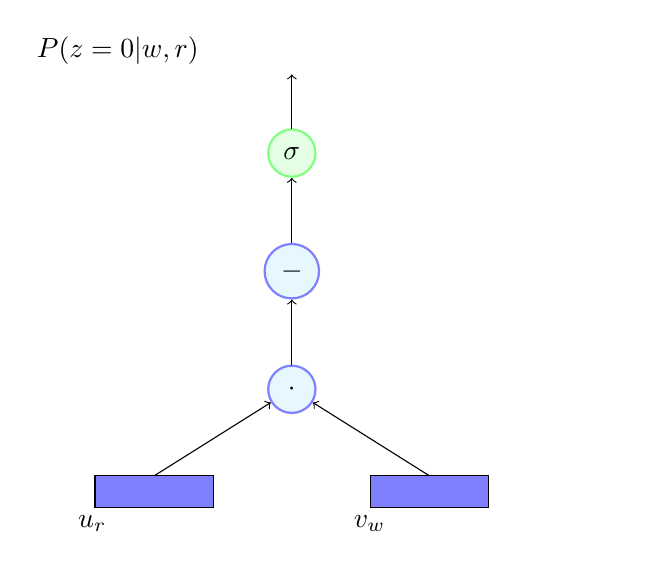
\begin{tikzpicture}
				\tikzstyle{hidden_neuron}=[circle,draw=blue!50,fill=cyan!10,thick,minimum size=6mm]
				\tikzstyle{output_neuron}=[circle,draw=green!50,fill=green!10,thick,minimum size=6mm]
				\node [hidden_neuron] (n1) at (0,1.5){$\cdot$};
				\node [hidden_neuron] (n2) at (0,3){$-$};
				\node [output_neuron] (n3) at (0,4.5){$\sigma$};
				\draw [->] (0,4.8) -- (0,5.5);
				\draw [->] (-1.75,0.4) -- (n1);
				\draw [->] (1.75,0.4) -- (n1);
				\node [text width=0.6\textwidth] at (0.4,5.8) {$P(z=0|w,r)$};
				\draw [->] (n1) -- (n2);
				\draw [->] (n2) -- (n3);
				\draw [fill=blue!50] (-2.5, 0) rectangle (-1,0.4);
				\draw [fill=blue!50] (1, 0) rectangle (2.5,0.4);
				\node [text width=0.2\textwidth] at (-1.5,-0.2){$u_{r}$};
				\node [text width=0.2\textwidth] at (2,-0.2){$v_w$};
			\end{tikzpicture}
		\end{overlayarea}
		\column{0.65\textwidth}
		\begin{overlayarea}{\textwidth}{\textheight}
			\footnotesize{\begin{itemize}
					\justifying
					\onslide<1->{\item Combining the two we get:}
					      \begin{align*}
						      \onslide<1->{  & \underset{\theta}{maximize}\underset{(w,c) \in D}{\prod}p(z=1|w,c) \underset{(w,r)\in D^{'}}{\prod}p(z=0|w,r)\\}
						      \onslide<2->{= & \underset{\theta}{maximize}\underset{(w,c) \in D}{\prod}p(z=1|w,c) \underset{(w,r)\in D^{'}}{\prod}(1- p(z=1|w,r))\\}
						      \onslide<3->{= & \underset{\theta}{maximize}\underset{(w,c) \in D}{\sum}\log p(z=1|w,c) \\
						       & \hspace{1cm}+ \underset{(w,r)\in D^{'}}{\sum}\log(1- p(z=1|w,r))\\}
						      \onslide<4->{= & \underset{\theta}{maximize}\underset{(w,c) \in D}{\sum}\log \frac{1}{1 + e^{-v_c^{T}v_w}} + \underset{(w,r)\in D^{'}}{\sum}\log \frac{1}{1 + e^{v_r^{T}v_w}}\\}
						      \onslide<5->{= & \underset{\theta}{maximize}\underset{(w,c) \in D}{\sum}\log \sigma(v_c^{T}v_w) + \underset{(w,r)\in D^{'}}{\sum}\log \sigma(-v_r^{T}v_w)}
					      \end{align*}
					      \onslide<5->{where $\sigma(x) = \frac{1}{1 + e^{-x}}$}
				\end{itemize}}
		\end{overlayarea}
	\end{columns}
\end{frame}


\begin{frame}
	\begin{columns}
		\column{0.35\textwidth}
		\begin{overlayarea}{\textwidth}{\textheight}
			\vspace{0.2in}
			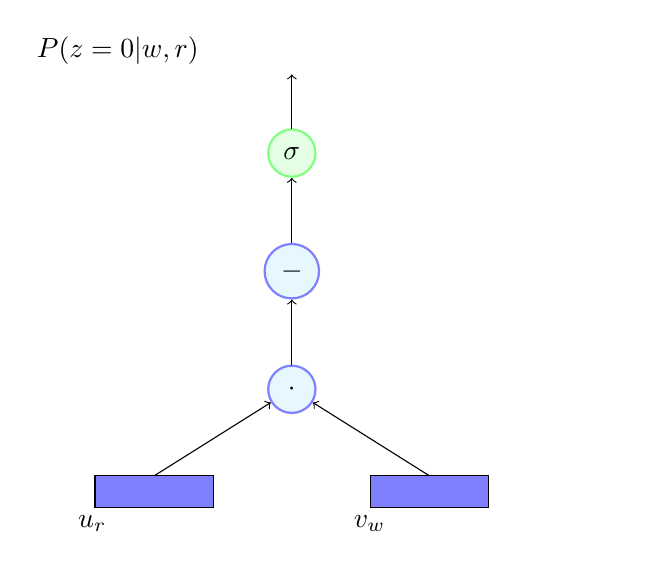
\begin{tikzpicture}
				\tikzstyle{hidden_neuron}=[circle,draw=blue!50,fill=cyan!10,thick,minimum size=6mm]
				\tikzstyle{output_neuron}=[circle,draw=green!50,fill=green!10,thick,minimum size=6mm]
				\node [hidden_neuron] (n1) at (0,1.5){$\cdot$};
				\node [hidden_neuron] (n2) at (0,3){$-$};
				\node [output_neuron] (n3) at (0,4.5){$\sigma$};
				\draw [->] (0,4.8) -- (0,5.5);
				\draw [->] (-1.75,0.4) -- (n1);
				\draw [->] (1.75,0.4) -- (n1);
				\node [text width=0.6\textwidth] at (0.4,5.8) {$P(z=0|w,r)$};
				\draw [->] (n1) -- (n2);
				\draw [->] (n2) -- (n3);
				\draw [fill=blue!50] (-2.5, 0) rectangle (-1,0.4);
				\draw [fill=blue!50] (1, 0) rectangle (2.5,0.4);
				\node [text width=0.2\textwidth] at (-1.5,-0.2){$u_{r}$};
				\node [text width=0.2\textwidth] at (2,-0.2){$v_w$};
			\end{tikzpicture}
		\end{overlayarea}
		\column{0.65\textwidth}
		\begin{overlayarea}{\textwidth}{\textheight}
			\begin{itemize}\justifying
				\onslide<1->{\item In the original paper, \textit{Mikolov et. al.} sample k negative $(w, r)$ pairs for every
				      positive $(w,c)$ pairs}
				      \onslide<2->{\item The size of $D^{'}$ is thus $k$ times the size of D}
				      \onslide<3->{\item The random context word is drawn from a modified unigram distribution} %raise to $\frac{3}{4}$
				      \onslide<4->{
					      \begin{align*}
						      r & \sim p(r)^{\frac{3}{4}}              \\
						      r & \sim \frac{count(r)^{\frac{3}{4}}}{N}
					      \end{align*}
					      $N$ = total number of words in the corpus}
			\end{itemize}
		\end{overlayarea}
	\end{columns}
\end{frame}
